%%%%%%%%%%%%%%%%%%%%%%%%%%%%%%%%%%%%%%%%%
%
% Optics and Radar -based observations
% EISCAT Space Weather Practical
%
%%%%%%%%%%%%%%%%%%%%%%%%%%%%%%%%%%%%%%%%%

%----------------------------------------------------------------------------------------
%	DOCUMENT CONFIGURATIONS
%----------------------------------------------------------------------------------------

\documentclass{article}

\title{\textbf {Optics and Radar Based Observations} \\ Practical\\ EISCAT ESR – incoherent scatter and weather in space} % Title
\def\authorivan{Ivan \v Sinkarenko}
\def\authoranu{Anuraj Rajendraprakash}
\author{\authorivan\\\authoranu}

\usepackage{graphicx}
\usepackage{fullpage}
\usepackage{url}
\usepackage{caption}
\usepackage{subcaption}

\begin{document}

\maketitle % Insert the title, author and date

\centerline{Referee: Dr. Victoria Barabash}

\setlength\parindent{0pt} % Removes all indentation from paragraphs

\renewcommand{\labelenumi}{\alph{enumi}.} % Make numbering in the enumerate environment by letter rather than number (e.g. section 6)
\clearpage

\tableofcontents

\listoffigures

\clearpage

%----------------------------------------------------------------------------------------
%	SECTION 1. Introduction
%----------------------------------------------------------------------------------------

\section{Introduction}
Space weather is the concept of changing environmental conditions in near-Earth space or the space from the Sun's atmosphere to the Earth's atmosphere. The observation of space weather is done both for scientific research and for applications. The type of observation done for science has varied over the years as the frontiers of our understanding has increased and due to competition for resources from other types of space-related research. The observations related to applications have been more systematic and has expanded over the years as awareness and applications have increased. \cite{Wiki:2012sw}\\
One of the ways to understand influence of space weather on near-Earth environment is to study ionosphere using incoherent scatter radar. A radar beam scattering off electrons in the ionospheric plasma creates an incoherent scatter return. The distribution function of the ionospheric electrons is modified by the much slower and massive positive ions — electron density fluctuations relate to ion temperature, mass distribution, and motion. The incoherent scatter signal allows measurement of electron density, ion temperature and electron temperatures, ion composition and plasma velocity. \cite{Wiki:2012is}
\\
The purpose of this laboratory experiment is to get acquainted with the EISCAT Svalbard Radar (ESR) system operating at frequency of 500 MHz. The transmitter/receiver of ESR is situated in Longyearbyen, Svalbard at 78$^{\circ}$09'11" N, 16$^{\circ}$01'44" E. Radar system has been run remotely with assistance from EISCAT staff. The main objective of the experiment is to understand how the ESR system works, which physical parameters can be studied in the data analysis and to compare the obtained results with space weather observations from other sources. \cite{Barabash:2011esr}

%----------------------------------------------------------------------------------------
%	SECTION 2. Experiment
%----------------------------------------------------------------------------------------

\section{Experiment}

The ESR is controlled by the EISCAT Realtime Operating System (EROS). This particular experiment comes with a codename "Beata".\\
The experiment took place at space campus near Kiruna, Sweden between 11:45 UT and 12:15 UT.
List of used commands during the experiment:
\begin{itemize}
\item \textbf{runexperiment /kst/exp/exp1 time now exp1}: (the full path must be given) at time time, which can be given at as \emph{HH:MM:SS} or \emph{now} or \emph{fullminute} etc.
\item \textbf{enablerecording}: Start recording data.
\item \textbf{disablerecording}: Stop recording data.
\item \textbf{stopexperiment}: Stop experiment immediately.
\end{itemize}
During the experiment data has been observed in real time with help of the real time graph software \emph{rtg}.

%----------------------------------------------------------------------------------------
%	SECTION 3. Data analysis and discussion
%----------------------------------------------------------------------------------------

\section{Data analysis and discussion}

After the experiment was performed the information about space weather was retrieved from the different sources. It was necessary to collect the relevant information from other sources to ensure that the experiment didn't go wrong and the data acquired is meaningful. For this reason Internet resources were used, including:
\begin{itemize}
\item \url{http://sohowww.nascom.nasa.gov/}
\item \url{http://www.swpc.noaa.gov/ace}
\item \url{http://www.spaceweather.com/}
\item \url{http://www.spacew.com/}
\end{itemize}
Later the data was combined to form the single impression of current space weather, including various solar wind parameters, sunspot number, magnetic field and plasma parameters.\\
\\
\textbf{Space weather for 2015-05-15 12:31 UT}:\\
\begin{tabular}{ l l }
Solar Wind speed:              & 396.2 $km/s$         \\
Solar Wind temperature:        & 42421.5 $K$          \\
Solar Wind density:            & 2.1 $particles/cm^3$ \\
Solar Wind pressure:           & 0.6 $nPa$            \\
Sunspots number:               & 72                   \\
Total Magnetic Field, B:       & 7.6 $nT$             \\
B-Field in x-direction, $B_x$: & 2.6 $nT$             \\
B-Field in y-direction, $B_y$: & -5.4 $nT$            \\
B-Field in z-direction, $B_z$: & 4.6 $nT$             \\
Latitude angle, $\beta$:       & 37.5$^{\circ}$       \\
Angle, $\theta$:               & 52.5$^{\circ}$       \\
\end{tabular}
\\
\\
\\
Also images were collected from different instruments of SOHO spacecraft, which made it clear that there were no any significant solar flares which could affect measurements at that time. The pictures are shown in Figure \ref{fig:SOHO}.

\begin{figure}[h!tb]
	\begin{subfigure}[b]{0.16\textwidth}
		\centering
		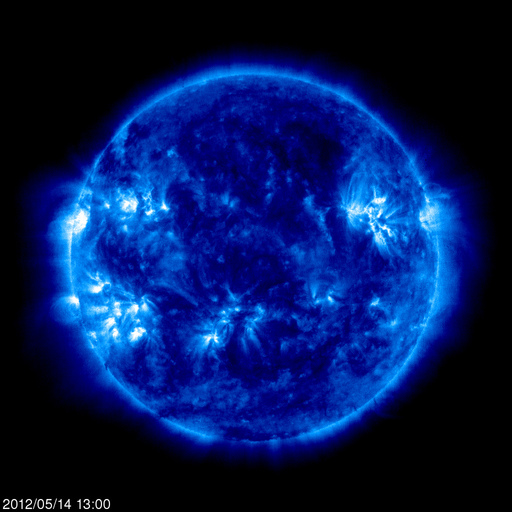
\includegraphics[width=\textwidth]{Figures/SOHOEIT171.jpg}
		\caption{EIT 171}
		\label{fig:SOHOEIT171}
	\end{subfigure}
	\begin{subfigure}[b]{0.16\linewidth}
		\centering
		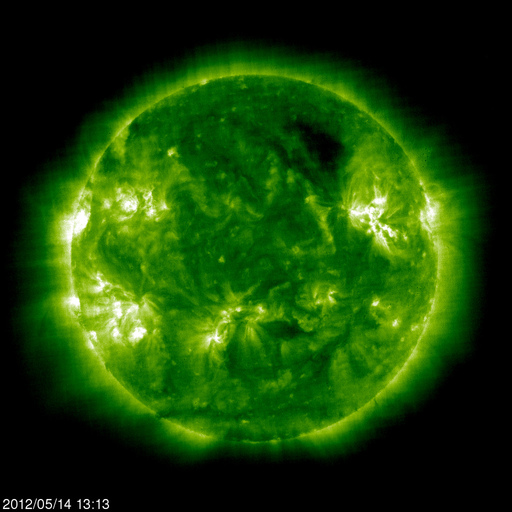
\includegraphics[width=\textwidth]{Figures/SOHOEIT195.jpg}
		\caption{EIT 195}
		\label{fig:SOHOEIT195}
	\end{subfigure}
	\begin{subfigure}[b]{0.16\linewidth}
		\centering
		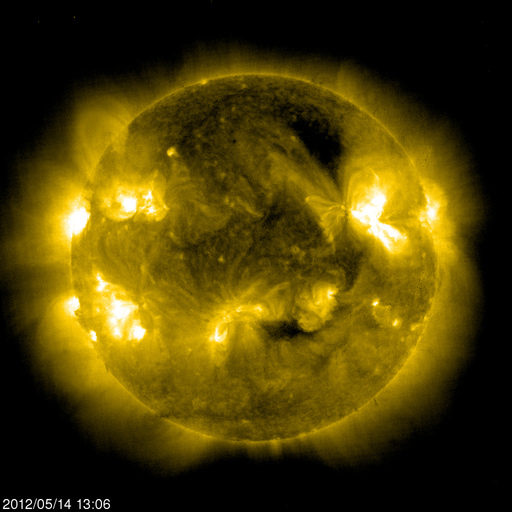
\includegraphics[width=\textwidth]{Figures/SOHOEIT284.jpg}
		\caption{EIT 284}
		\label{fig:SOHOEIT284}
	\end{subfigure}
	\begin{subfigure}[b]{0.16\linewidth}
		\centering
		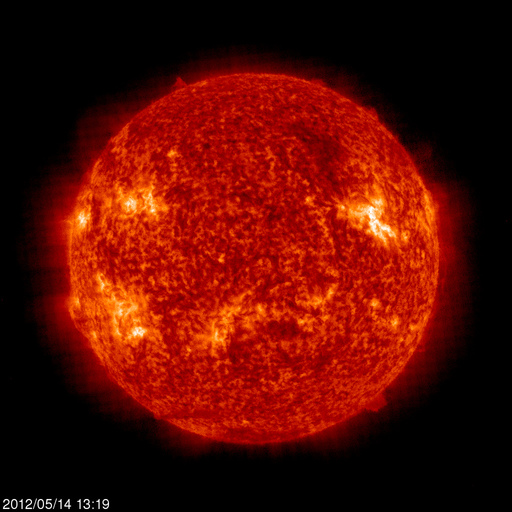
\includegraphics[width=\textwidth]{Figures/SOHOEIT304.jpg}
		\caption{EIT 304}
		\label{fig:SOHOEIT304}
	\end{subfigure}
	\begin{subfigure}[b]{0.16\linewidth}
		\centering
		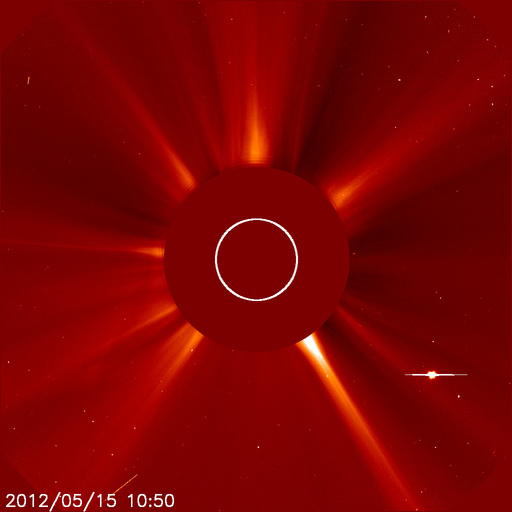
\includegraphics[width=\textwidth]{Figures/SOHOLASCOC2.jpg}
		\caption{LASCO C2}
		\label{fig:SOHOLASCOC2}
	\end{subfigure}
	\begin{subfigure}[b]{0.16\linewidth}
		\centering
		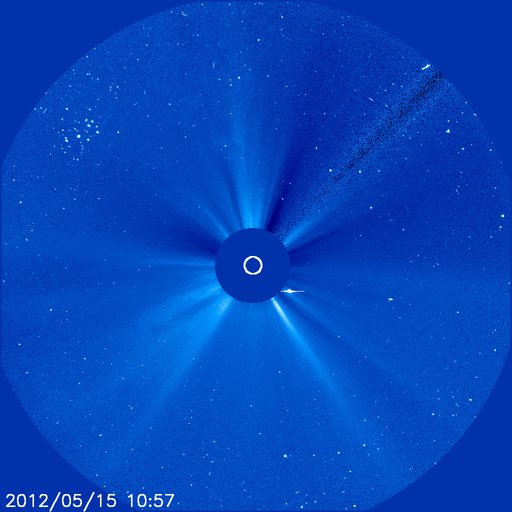
\includegraphics[width=\textwidth]{Figures/SOHOLASCOC3.jpg}
		\caption{LASCO C3}
		\label{fig:SOHOLASCOC3}
	\end{subfigure}
	\caption{SOHO instrument images}
	\label{fig:SOHO}
\end{figure}

%----------------------------------------------------------------------------------------
%	SECTION 4. Data analysis and discussion
%----------------------------------------------------------------------------------------

\section{Conclusion}

%----------------------------------------------------------------------------------------
%	SECTION 5. REFERENCES
%----------------------------------------------------------------------------------------
\newpage
\begin{thebibliography}{9}

\bibitem{Wiki:2012sw}
Wikipedia.org. (2012).
\newblock {\em Space weather}.
\newblock {\url{http://en.wikipedia.org/wiki/Space_weather}}.

\bibitem{Wiki:2012is}
Wikipedia.org. (2012).
\newblock {\em Incoherent scatter}.
\newblock {\url{http://en.wikipedia.org/wiki/Incoherent_scatter}}.

\bibitem{Barabash:2011esr}
EISCAT HQ / Barabash V. (2011).
\newblock {\em Practical. EISCAT ESR – incoherent scatter and weather in space}.
\newblock Lule\aa \ University of Technology, Kiruna, Sweden.

\bibitem{Skolnik:2001irs}
Skolnik M. ~I.  (2001).
\newblock {\em Introduction to Radar Systems}.
\newblock The McGraw-Hill Companies, Inc., New York, United States.

\bibitem{Rottger:2000ip}
R\"ottger J.  (2000).
\newblock {\em The Instrumental Principles of MST Radars and Incoherent Scatter Radars and The Configuration of Radar System Hardware}.
\newblock Max Planck Institut F\"ur Aeronomie, Katlenburg-Lindau, Germany.


\end{thebibliography}

%----------------------------------------------------------------------------------------
%	SECTION 6. Confirmation
%----------------------------------------------------------------------------------------
\newpage
\section{Confirmation of Participation}

This is to confirm that the members of this team participated on the investigation of the required information to solve the assignment, generated their code to perform the calculation and discussed the results.\\
\vspace{2cm}
\newline
\line(1,0){200}\\
\authorivan\\
\vspace{2cm}
\newline
\line(1,0){200}\\
\authoranu\\


\end{document}